\documentclass[10pt]{beamer}

\usetheme{Montpellier}
\usecolortheme{whale}

\usepackage[T1]{fontenc}
\usepackage{lmodern}

\usepackage{mathtools}
\usepackage[binary-units]{siunitx}
\usepackage{amsmath}
\usepackage{listings}
\usepackage{mdframed}
\usepackage{adjustbox}
\usepackage{minted}
\usepackage{xcolor}

\usepackage{parskip}
\usepackage{substr}
\usepackage{hyperref}
\usepackage{etoolbox}
\usepackage{tipa}
\usepackage{cprotect}
\usepackage{booktabs}
\usepackage{silence}
\usepackage[backend=biber, style=ieee]{biblatex}
\usepackage[english,ngerman]{babel}
\usepackage{csquotes}

\definecolor{lg}{gray}{0.95}
\hypersetup{colorlinks = true, urlcolor=blue, linkcolor=white}
\WarningFilter{biblatex}{Patching footnotes failed}

\renewcommand*{\bibfont}{\tiny}
\renewcommand{\subsectionname}{AA}

\bibliography{resources.bib}

\title{\textbf{Operating Systems}}
\subtitle{Tutorial 8}
\author{Fabian Klopfer}
\date{\today}

\defbeamertemplate{subsection page}{mine}[1][]{%
  \begin{centering}
    {\usebeamerfont{subsection name}\usebeamercolor[fg]{subsection name}#1}
    \vskip1em\par
    \begin{beamercolorbox}[sep=12pt,center]{part title}
      \usebeamerfont{subsection title}\insertsubsection\par
    \end{beamercolorbox}
  \end{centering}
}

\defbeamertemplate{section page}{mine}[1][]{%
  \begin{centering}
    {\usebeamerfont{section name}\usebeamercolor[fg]{section name}#1}
    \vskip1em\par
    \begin{beamercolorbox}[sep=12pt,center]{part title}
      \usebeamerfont{section title}\insertsection\par
    \end{beamercolorbox}
  \end{centering}
}

\setbeamertemplate{section page}[mine]
\setbeamertemplate{subsection page}[mine]

\begin{document}
\frame{\titlepage}


\begin{frame}{Intro}
\begin{itemize}
 \item Pingo Polls
 \item No new exercise sheet this week
 \item Loaders: The broad context \& Linking
\end{itemize}
\end{frame}

\section*{Exercise Sheet 7}
\frame{\sectionpage}
\subsection*{Exercise 1}
\frame{\subsectionpage}
\begin{frame}[allowframebreaks, fragile]{Exercise 1}
    \begin{enumerate}
		\item How could virtualization on a desktop computer be useful to developers? \\
		\alert{
		\begin{itemize}
		 \item Testing
		 \item Avoid dual boot setups
		 \item Security through isolation: QubesOS
		\end{itemize}
		}
		\framebreak
        \begin{figure}
            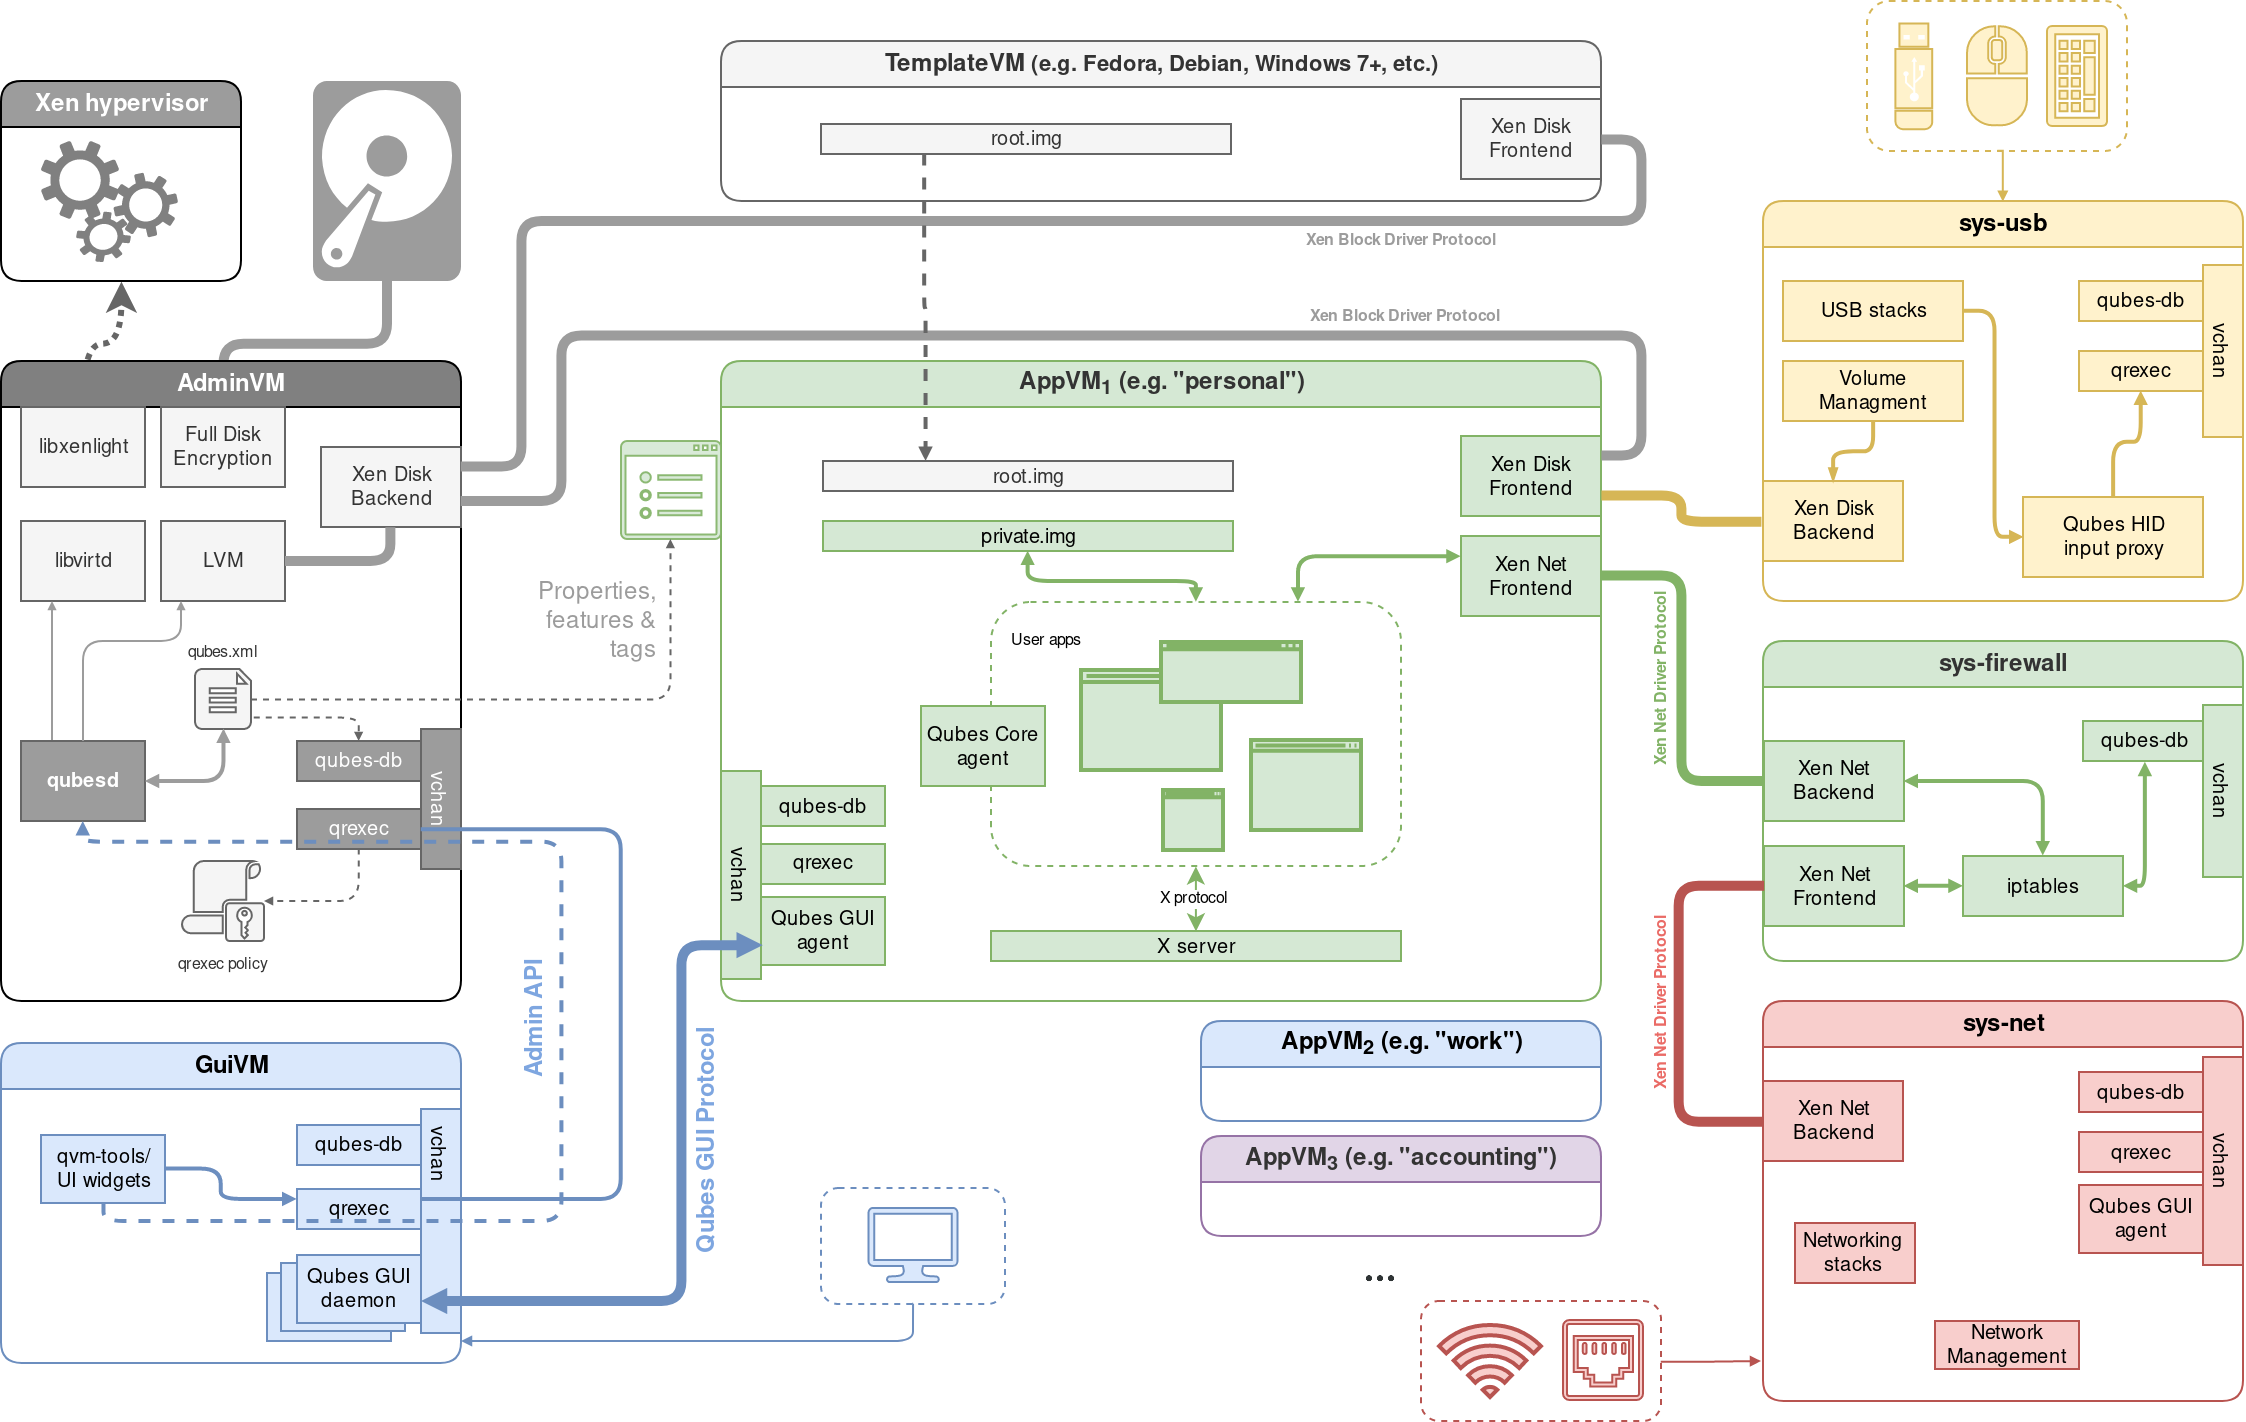
\includegraphics[keepaspectratio, width=\textwidth, height=\textheight-2\baselineskip-2\baselineskip]{img/qubesos.png} \\
        \end{figure}
		\framebreak
		
		\item Which of the following instruction groups is not sensitive in the sense of Popek \& Goldberg (1974)? \\
		\begin{enumerate}
		 \item Instructions that access the memory management unit (MMU), 
		 \item instructions that access the input/output MMU (I/O MMU),
		 \item instructions that access the Arithmetic-Logical Unit (ALU).
		\end{enumerate}
		\alert{instructions that access the Arithmetic-Logical Unit (ALU).}
		
		
		\item What is a privileged instruction in the sense of Popek \& Goldberg (1974)?\\
		\alert{Privileged instructions hand over the control to the OS via a trap.}
		
		\item Can a hypervisor virtualize more operating systems than there are (hard)disk partitions in the computing system? Why? \\
		\alert{Yes, hypervisors can create an arbitrary number of Subpartitions}
		
		\item Give an example in the context of virtualization where binary translation can be faster than the original code.\\
		\alert{Clear Interrupt instructions: \\
		\begin{itemize}
		 \item On HW: trap to hypervisor
		 \item Using BAT: Changing a flag in memory
		\end{itemize}
        }
		
		\item What is the main problem with virtualization and memory?\\
		\alert{Multiple Guests allocate frame $k$ at the same time $\Rightarrow$ Problem \\
            Solution: Another page table/mapping: Guest frame to Hypervisor/actual frame}
		
		\item What problem does the hypervisor face when it wants to evict a page of a virtualized operating system? \\
		\alert{May evict page that is frequently used by guest.}
		
		\item What is the purpose of balloon drivers? \\
		\alert{Hypervisor does not know page usage of guests \\
            Workasrround: Balloon drivers in the guests. \\
            If hypervisor runs out of space the ballon driver increases its memory usage, forcing the guest to evict a page.}
	\end{enumerate}
\end{frame}

\subsection*{Exercise 2}
\frame{\subsectionpage}
\begin{frame}[allowframebreaks, fragile]{Exercise 2}
    	\begin{enumerate}
		\item What does \mintinline{c}{int * const p1;} declare? \\ \vspace{0.3cm}
		\alert{Unchangeable pointer that can be used to change the pointed-to integer.}
		
		\item What does \mintinline{c}{int const * p2;} declare? \\ \vspace{0.3cm}
			\alert{A changable pointer that cannot be used to change the pointed to integer.\\
			Same as \mintinline{c}{const int* p2}}
			
		\item What does \mintinline{c}{int (*p3)[3];} declare?\\ \vspace{0.3cm}
		\alert{Pointer to an array of 3 integers.}
		
		\item What does \mintinline{c}{float f1(int const * p);} declare? \\ \vspace{0.3cm}
		\alert{A function that returns a float, taking a pointer to an unchangeable integer as argument.}
		
		\item Is the function signature \mintinline{c}{void f2(int * const p);} meaningful? Why? \\ \vspace{0.3cm}
		\alert{As pointers are passed by value (the object they point to are passed by reference), a local variable within the scope of the function is created. By the const one cannot change where the pointer points to. The local variable can not be changed. Meaningful? Sort of, but not really.}
		
		\item%
			What is the problem in the following code snippet?
			\begin{minted}[autogobble]{c}
void f(char *p) { *p = 'x'; }
...
f("Hello world!");
            15:\end{minted} 
			\alert{``Hello World'' is a compile time constant, i.e. it will be put into the binary/code segment of the process which is \textbf{read-only}. \\
			Changing it as in f() segfaults}
			
		\item Declare a function that returns a pointer to an \mintinline{c}{int} array with 3 elements and accepts no arguments. \\ \vspace{0.3cm}
			\alert{\mintinline{c}{int (*f(void))[3];}}
			
		\item Declare a pointer to this function. \\ \vspace{0.3cm}
			\alert{\mintinline{c}{int (*(*p4)(void))[3];}}
			
	\end{enumerate}
\end{frame}

\subsection*{Exercise 3}
\frame{\subsectionpage}
\begin{frame}[allowframebreaks, fragile]{Exercise 3}
    A \emph{palindrome} is a string which is the same when read forwards or backwards:
	\[ \forall i=1,\ldots,|s| : s_i = s_{|s|-i+1} \]
	Where $|s|$ denotes the length of the string~$s$.
	Write a function with the signature \mintinline{c}{int is_palindrome(char const* s)} that tests whether a string is a palindrome.
	
	 \adjustbox{varwidth=\textwidth, scale=0.7}{\inputminted{c}{code/palindrome.c}}
\end{frame}

\subsection*{Exercise 4}
\frame{\subsectionpage}
\begin{frame}[allowframebreaks,fragile]{Christmas animation}
 Write a program that outputs a seasonally appropriate animation to the text console,
	for example, a landscape with snow falling.
	
	\adjustbox{varwidth=\textwidth, scale=0.5}{\inputminted{c}{code/main.c}} \\
	\framebreak
	\adjustbox{varwidth=\textwidth, scale=0.7}{\inputminted{c}{code/simulate_timestep.c}} \\
	\framebreak
	\adjustbox{varwidth=\textwidth, scale=0.7}{\inputminted{c}{code/print_frame.c}} \\
\end{frame}

    
\section*{Loader}
\frame{\sectionpage}
\begin{frame}[allowframebreaks, fragile]{}
    We want to know what happens when we run code exactly. \\
    First we write some code: \vspace{0.35cm} \\ 
    \adjustbox{varwidth=\textwidth, scale=0.7}{\inputminted{c}{code/hello_world.c}} \vspace{0.35cm} \\	
    We compile it:  \\ 
    \begin{minted}{c}
    gcc hello_world.c -o hello
    \end{minted}
    \framebreak
    
    What actually happens:
    \begin{figure}
        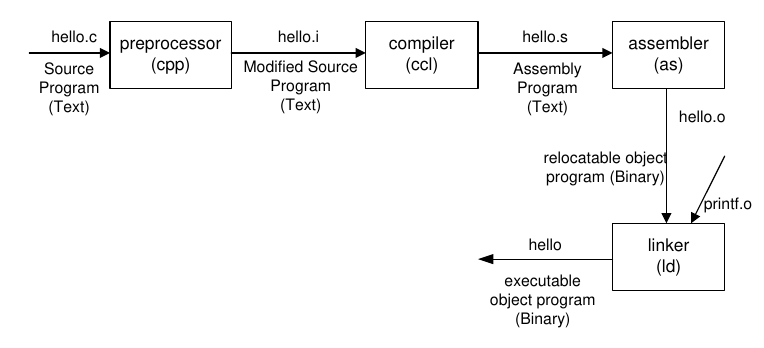
\includegraphics[keepaspectratio, width=0.8\textwidth, height=\textheight-2\baselineskip-2\baselineskip]{img/compile.png} \\
    \end{figure}
    The assembler produces binary code in ``Executable and Linking Format'' (ELF) ... \\
    \framebreak
    Which looks like this:
    \begin{figure}
        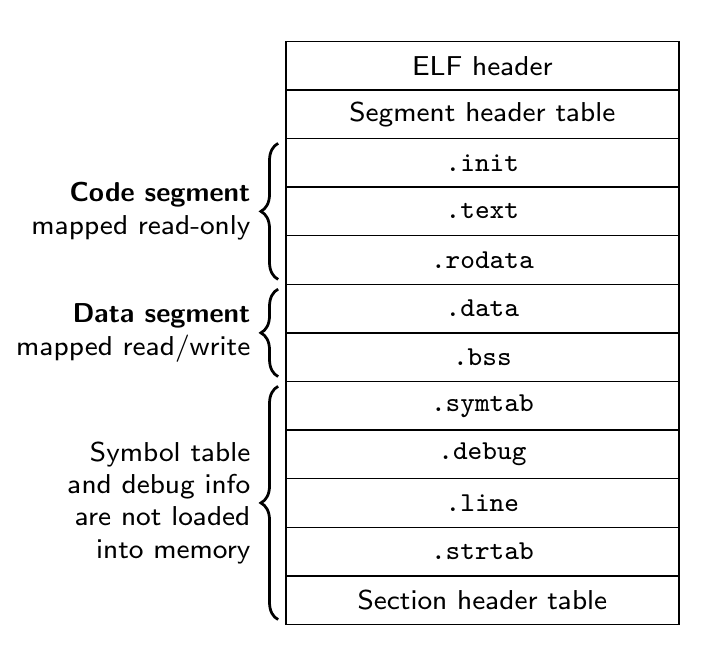
\includegraphics[keepaspectratio, width=\textwidth, height=\textheight-2\baselineskip-2\baselineskip]{img/elf.png} \\
    \end{figure}
    \framebreak
    
     What does the linker actually do? \\
     
    Given: A file in ELF format with unresolved symbols and paths to libraries$^1$ \\
    Desired: A file in ELF format with resolved symbols. \\
    What it does: Scan the files for the appropiate symbol and replace it accordingly.
    \begin{figure}
        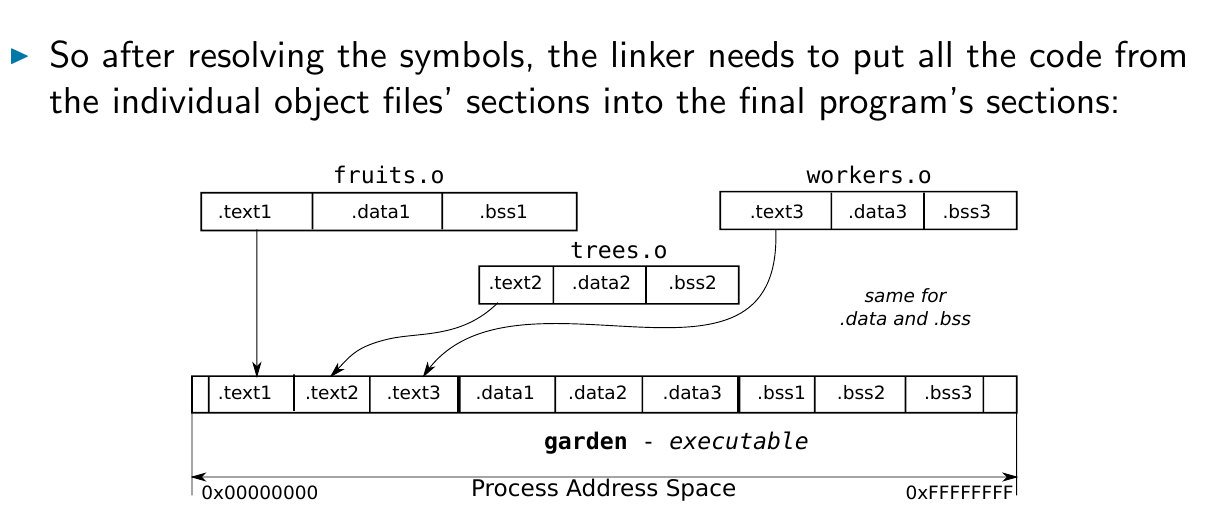
\includegraphics[keepaspectratio, width=0.8\textwidth, height=\textheight-2\baselineskip-2\baselineskip]{img/reloc.png} \\
    \end{figure}
    
    \begin{tiny}
     $^1$defaults: \mintinline{bash}{/lib, /usr/lib}
    \end{tiny}

    \framebreak
    
    Taking a closer look at (the relevant part of) the .text section: \\
    \adjustbox{varwidth=\textwidth, scale=0.8}{\inputminted{c}{code/hello_world.s}} \vspace{0.35cm} \\  
    We can see that puts is called. If we look at the symbol table (.symtab) we notice: \\
    \adjustbox{varwidth=\textwidth, scale=0.8}{\inputminted{c}{code/hello_world.sym}} \vspace{0.55cm} \\  
    \mintinline{c}{puts} is undefined after linking! \\
    \framebreak
   
    
    But wait! We linked it and \mintinline{c}{puts} is still undefined?! \vspace{0.35cm}  \\
    Yes it is and that's totaly fine: \vspace{0.35cm} \\
    Executables vs. Static libraries (\mintinline{bash}{.a}) vs. shared libraries (\mintinline{bash}{.so}) \vspace{0.35cm}  \\
    \begin{figure}
        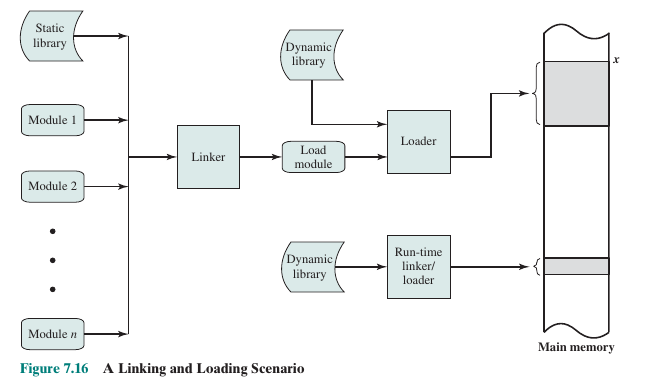
\includegraphics[keepaspectratio, width=\textwidth, height=0.8\textheight-2\baselineskip-2\baselineskip]{img/linker_loader.png} \\
    \end{figure}
    \framebreak
    
    More comprhensive linking description: Programming slides, last section
    Thus distingiush between static and dynamic executables. \vspace{0.35cm}  \\
    Our hello executable is a dynamic executable: \vspace{0.35cm} \\
    \adjustbox{varwidth=\textwidth, scale=0.7}{\inputminted{c}{code/hello_world.file}}  \vspace{0.35cm} \\
    The Linnker just marks what's to be done for the loader:  \vspace{0.35cm}  \\
    \adjustbox{varwidth=\textwidth, scale=0.7}{\inputminted{c}{code/hello_world.annot}} \\
    \framebreak
    
    Linkers link static libraries and other source files.  \\
    Additionally they mark symbols from dynamic libraries for the loader. \vspace{0.5cm}  \\
    The Loader links dynamic libraries/shared objects/dlls, previously marked by the linker  \vspace{0.9cm} \\
    But what about the rest?
    \framebreak
    
    Lets execute our elf file: \mintinline{c}{./hello}\\
    What happens under the hood of the shell is (pseudo code)
    \begin{minted}{c}
     switch(pid = fork()) {
        case -1: 
            exit(-1);
            
        case 0: // child
            execve("./hello", NULL, NULL);
            exit(0);
            
        default: // parent
            waitpid(pid)
     }
    \end{minted}
    I.e. copy the process image using fork and replace the relevant stuff using execve
    \framebreak
    
    The \mintinline{c}{execve} system call builds a an instanct of the \mintinline{c}{binprm} struct \vspace{0.35cm} \\
    Then iterates over available binary handlers using \mintinline{c}{search_binary_handler}. \vspace{0.35cm}\\
    Besides ELF there are handlers for e.g. scripts and jars \\
    Finally \mintinline{c}{load_elf_binary(struct binprm* bin)} is called. \vspace{0.35cm} \\
    
    \textbf{To be continued}
    
\end{frame}

\section{References}
    \begin{frame}[allowframebreaks]
      \frametitle{References}
      \begin{tiny}
      \nocite{*}
      \printbibliography
      \end{tiny}
    \end{frame}


\end{document}
 
